\documentclass[12pt, letterpaper]{report}
\usepackage[margin=1in]{geometry}
\usepackage[utf8]{inputenc}
\usepackage{graphicx}
\usepackage{float}
\usepackage{subfig}
\graphicspath{ {./img/} }
\setlength\parindent{0pt}
\renewcommand\thesection{\arabic{section}.}
\renewcommand{\thesubsection}{(\alph{subsection})}


\title{ECE1166 - OpenMP Analysis}
\author{Zachary M. Mattis}


\begin{document}
	
\maketitle


\section{Shared-Memory Multiprocessing}

OpenMP allows distributed sharing of workload spread across different processing elements. OpenMP is a directive-driven programming model, where compiler instructions dictate how the running program is to be split across multiple processors. The running process is forked via OpenMP, which duplicates the currently active instruction set, allowing different processors to independently complete their assigned work. At the end of these regions, the processes rejoin into a master thread that continues the completion of the application. However, with different resources running the same code, their are instances in which these different processes can become out of sync. Through the use of barriers, OpenMP specifies locations where each processor must wait for everyone to finish their assigned work before continuing. This barrier sync is used to avoid race conditions, which are instances in which the behavior of a system can change on subsequent executions depending on the completion rate of different, heterogeneous processing elements.
\\ \\
Considering that OpenMP is a shared-memory processing paradigm, the regions of work include both shared and private variables. Shared variables allow for only 1 instance of memory that can be utilized between each of the running threads, reducing the memory overhead. However, this can become problematic if a processor modifies this location, as it can become out of sync with the other processing elements relying on it. Private memory is used by each individual processing element and can not be seen by the other threads. This type of memory is useful for the intermediary work of the individual threads. Upon creation of the threads, work must be divided among them, a process known as scheduling. Two main methods, static and dynamic, are used to distribute this work. Static scheduling occurs during compile-time to assign equally-distributed work to each thread. Dynamic scheduling occurs at run-time and assigns additional work to open processors. Dynamic scheduling has overhead during run-time because scheduling decisions need to be calculated, but this can be an advantage over static scheduling when using heterogeneous resources that take different lengths of time to complete their assigned work.


\section{Thread Management}

\begin{verbatim}

1. omp_get_thread_num()  - get the thread rank in a parallel region
2. omp_get_num_threads() - get the number of threads used in a parallel region
3. omp_get_max_threads() - get the maximum number of OpenMP threads available

\end{verbatim}

\section{Compiler Directive Parameters}

\begin{verbatim}
1. private     - variables used exclusively by each thread
2. shared      - variables shared between threads
3. default     - default for variables not specified in private/shared
4. num_threads - number of threads to be used in parallel region
5. schedule    - how work is to be divided among processing elements
\end{verbatim}

\section{Parallel Computation}

% A
\subsection{Serial Execution}

The compiler directive 
\begin{verbatim}#pragma omp single { ... }\end{verbatim}
is used to indicate that the following block of code is to be executed by only 1 processing element, ensuring that it will be executed serially.

% B
\subsection{Block vs. Cyclic Decomposition}

Block and Cyclic parallelization are methods of data decomposition for dividing a problem. An advantage of block division is that a processor has access to contiguous pieces of data, which is especially important in instances where the computation has dependencies upon corresponding, neighboring data.

% C
\subsection{Domain vs. Functional}

Domain and Functional decomposition are two differing methods for dividing a problem for parallelization. In domain decomposition, the primary focus is on the how the data for the computations is to be spit between processing elements. This differs from functional decomposition, where the emphasis is placed on the computation itself, in which the overall function is broken down into smaller, simplified calculations.

% D
\subsection{Critical vs. Atomic}

Critical sections are general sections used to provide mutual exclusion of a given section. They are often used to prevent concurrent access to limited computer resource such as a peripheral device, ensuring that only 1 thread has access to it at a time. Atomic sections have far less overhead and often rely on the hardware to supply an atomic operation, such as checking the value of a lock (bit) and setting its value in the same clock cycle.


\section{Matrix Multiplication}

\begin{table}[H]
	\centering
	\begin{tabular}{ |l|l|l|l|l| }
		\hline
		\textbf{Matrix Size} & \textbf{Num Procs} & \textbf{Exec Time(s)} & \textbf{Speed Up} & \textbf{Efficiency} \\
		\hline \hline \hline
		(10x10) * (10x10) & Serial & 0.001060 & - & - \\
		\hline
		(10x10) * (10x10) & 1 & 0.001227 & 0.8638956 & 0.8638956 \\
		\hline
		(10x10) * (10x10) & 2 & 0.0012658 & 0.8374150 & 0.4187075 \\
		\hline
		(10x10) * (10x10) & 4 & 0.0015758 & 0.6726741 & 0.1681685 \\
		\hline
		(10x10) * (10x10) & 8 & 0.0010804 & 0.9811181 & 0.1226397 \\
		\hline
		(10x10) * (10x10) & 16 & 0.001271 & 0.8339889 & 0.0521243 \\
		\hline \hline \hline
		(100x100) * (100x100) & Serial & 0.001496 & - & - \\
		\hline
		(100x100) * (100x100) & 1 & 0.001589 & 0.941472624 & 0.941472624 \\
		\hline
		(100x100) * (100x100) & 2 & 0.0013778 & 1.0857889 & 0.5428944 \\
		\hline
		(100x100) * (100x100) & 4 & 0.0011728 & 1.2755798 & 0.3188949 \\
		\hline
		(100x100) * (100x100) & 8 & 0.0012608 & 1.1865482 & 0.1483185 \\
		\hline
		(100x100) * (100x100) & 16 & 0.001379 & 1.084844 & 0.0678027 \\
		\hline \hline \hline
		(1000x1000) * (1000x1000) & Serial & 0.666 & - & - \\
		\hline
		(1000x1000) * (1000x1000) & 1 & 0.0012658 & 0.9580214 & 0.9580214 \\
		\hline
		(1000x1000) * (1000x1000) & 2 & 0.0015758 & 1.6661021 & 0.8330510 \\
		\hline
		(1000x1000) * (1000x1000) & 4 & 0.0010804 & 3.7909533 & 0.9477383 \\
		\hline
		(1000x1000) * (1000x1000) & 8 & 0.001227 & 7.8733827 & 0.9841728 \\
		\hline
		(1000x1000) * (1000x1000) & 16 & 0.001271 & 9.6226366 & 0.6014147 \\
		\hline
	\end{tabular}
	\caption{Matrix Multiplication Analysis}
\end{table}

OpenMP's parallelization of the matrix multiply shows the speedup in program execution, especially highlighted by the large matrix size of 1000. The table above shows improved speedup and efficiency as the size of the matrix increases. Due to the overhead of setting up the parallel threads, smaller matrices display much less speedup and efficiency when compared to much larger sizes. When the size is small enough, using multiple processors can even result in slowdown due to large overhead when the number of computations is minimal.

\section{Mandelbrot}

Each Mandelbrot set was testing using an image height x width of 2048 x 2048 pixels.

\begin{table}[H]
	\centering
	\begin{tabular}{ |l|l| }
		\hline
		\textbf{Scheduling, Chunk Size} & \textbf{Execution Time (ms)} \\
		\hline
		Static, Typical &  545.9812 \\
		\hline
		Static, 10 & 382.7061 \\
		\hline
		Static, 100 & 358.7033 \\
		\hline
		Static, 2 & 376.6455 \\
		\hline
		Dynamic, Typical & 372.7525 \\
		\hline
		Dynamic, 10 & 337.2467 \\
		\hline
		Dynamic, 100 & 352.3983 \\
		\hline
		Dynamic, 2 & 343.0696 \\
		\hline
		Guided & 323.733 \\
		\hline
	\end{tabular}
	\caption{Scheduling}
\end{table}


\begin{figure}[H]
	\centering
	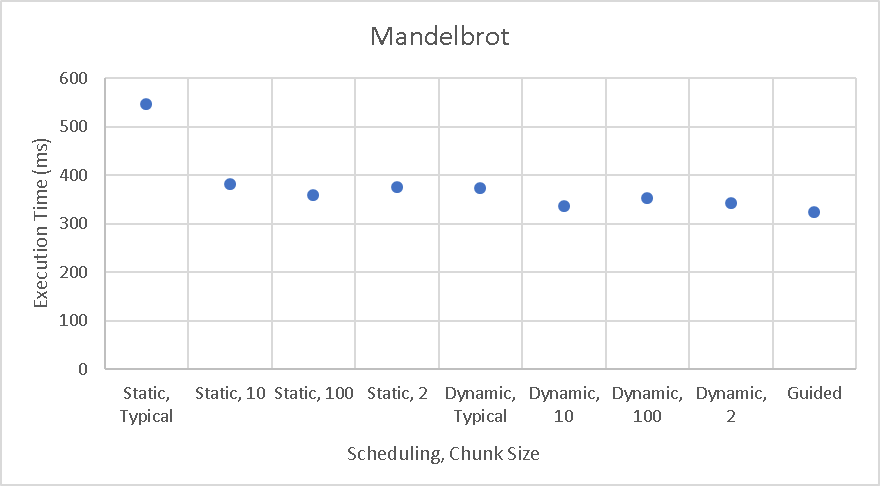
\includegraphics[width=0.7\columnwidth]{mandelbrot.png}
	\caption{Data Decomposition}
\end{figure}

Figure 1 above shows the execution time of the Mandelbrot set using various scheduling algorithms. The majority of scheduling algorithms did not demonstrate major differences in computation time, but did show that there are minor differences in execution time dependent upon how the work is divided. Overall, dynamic scheduling appeared to produce better timing than the static scheduling, implying that by redistributed work to idle processors, the execution of the program can be reduced. Additionally, the guided scheduling produced the quickest time, as expected. This hybrid approach reduces the chunk size of dynamically distributed work to different threads as the program runs, thus decreasing uneven distribution of work and providing the best load-balancing between all of the processing elements.

\section{Conway's Game of Life}

The C implementation of Conway's Game of Life was parallelized via a ``Block, *" data decomposition, as illustrated in Figure 1. This type of decomposition assigns a contiguous block of rows to each processing element, where independent calculations are made upon each cell to determine its surrounding neighbor count. This implementation utilizes a mesh grid, wherein each node only considers its physical neighbors and NOT corresponding opposite edge nodes for those nodes located on the edge of the grid. Additionally, memory is organized using row-major order as a contiguous array for a 2-D array of char's (bytes).

\begin{figure}[H]
	\centering
	
\includegraphics[width=0.3\columnwidth]{block.png}
	\caption{Scheduling}
\end{figure}


\begin{table}[H]
	\centering
	\begin{tabular}{ |l|l|l|l|l|l| }
		\hline
		\textbf{Iterations} & \textbf{Grid Size} & \textbf{Num Procs} & \textbf{Exec Time(s)} & \textbf{Speed Up} & \textbf{Efficiency} \\
		\hline \hline \hline
		100 & 10 x 10 & Serial & 0.001 & - & - \\
		\hline
		100 & 10 x 10 & 1 & 0.004746 & 0.2107037 & 0.2107037 \\
		\hline
		100 & 10 x 10 & 2 & 0.005203 & 0.192196 & 0.0960984 \\
		\hline
		100 & 10 x 10 & 4 & 0.004945 & 0.202224469 & 0.0505561 \\
		\hline \hline \hline
		100 & 100 x 100 & Serial & 0.01 & - & - \\
		\hline
		100 & 100 x 100 & 1 & 0.033093 &  0.3021787 & 0.3021787 \\
		\hline
		100 & 100 x 100 & 2 & 0.021576 & 0.4634779 & 0.2317389 \\
		\hline
		100 & 100 x 100 & 4 & 0.013651 & 0.732547066 & 0.1831367 \\
		\hline \hline \hline
		100 & 1000 x 1000 & Serial & 1.31 & - & - \\
		\hline
		100 & 1000 x 1000 & 1 & 1.392049 & 0.9410588 & 0.9410588 \\
		\hline
		100 & 1000 x 1000 & 2 & 1.070155 & 1.2241217 & 0.612060 \\
		\hline
		100 & 1000 x 1000 & 4 & 0.854598 & 1.5328844 & 0.3832211 \\
		\hline \hline \hline
		100 & 10 x 1000 & Serial & 0.01 & - & - \\
		\hline
		100 & 10 x 1000 & 1 & 0.02369 & 0.4221190 & 0.4221190 \\
		\hline
		100 & 10 x 1000 & 2 & 0.016278 & 0.6143260 & 0.3071630 \\
		\hline
		100 & 10 x 1000 & 4 & 0.015317 & 0.6528693 & 0.163217 \\
		\hline \hline \hline
		100 & 1000 x 10 & Serial & 0.01 & - & - \\
		\hline
		100 & 1000 x 10 & 1 & 0.019232 & 0.5199667 & 0.519966722 \\
		\hline
		100 & 1000 x 10 & 2 & 0.017046 & 0.5866478 & 0.2933239 \\
		\hline
		100 & 1000 x 10 & 4 & 0.013713 & 0.7292350 & 0.1823087 \\
		\hline
	\end{tabular}
	\caption{Grid Size Analysis}
\end{table}


\begin{table}[H]
	\centering
	\begin{tabular}{ |l|l|l|l|l|l| }
		\hline
		\textbf{Iterations} & \textbf{Grid Size} & \textbf{Num Procs} & \textbf{Exec Time(s)} & \textbf{Speed Up} & \textbf{Efficiency} \\
		\hline \hline \hline
		10 & 10 x 10 & Serial & 0.001 & - & - \\
		\hline
		100 & 10 x 10 & Serial & 0.01 & - & - \\
		\hline
		1000 & 10 x 10 & Serial & 0.1 & - & - \\
		\hline
		10000 & 10 x 10 & Serial & 0.99 & - & - \\
		\hline \hline \hline
		10 & 10 x 10 & 1 & 0.007182 & 0.1392369 & 0.1392369 \\
		\hline
		100 & 10 x 10 & 1 & 0.01922 & 0.5202913 & 0.5202913 \\
		\hline
		1000 & 10 x 10 & 1 & 0.118198 & 0.8460380 & 0.8460380 \\
		\hline
		10000 & 10 x 10 & 1 & 1.061191 & 0.9329140 & 0.9329140 \\
		\hline \hline \hline
		10 & 10 x 10 & 2 & 0.008745 & 0.8212692 & 0.4106346 \\
		\hline
		100 & 10 x 10 & 2 & 0.01651 & 1.1641429 & 0.5820714 \\
		\hline
		1000 & 10 x 10 & 2 & 0.091448 & 1.2925159 & 0.6462579 \\
		\hline
		10000 & 10 x 10 & 2 & 0.817902 & 1.2974549 & 0.6487274 \\
		\hline \hline \hline
		10 & 10 x 10 & 4 & 0.007112 & 1.2296119 & 0.3074029 \\
		\hline
		100 & 10 x 10 & 4 & 0.014072 & 1.1732518 & 0.2933129 \\
		\hline
		1000 & 10 x 10 & 4 & 0.073683 & 1.241100 & 0.3102750 \\
		\hline
		10000 & 10 x 10 & 4 & 0.67535 & 1.2110787 & 0.3027696 \\
		\hline
	\end{tabular}
	\caption{Iterations Analysis}
\end{table}


The testing of Conway's Game of Life was tested using a display frequency of 10. Overall, Conway's Game did not demonstrate nearly as much parallelization speed up and efficiency as the previous matrix multiply. This is expected, as the overhead of context switching to constantly print the grid to standard out greatly slows down the execution of the program. The entire printing of the matrix must be done sequentially as to correctly display the Conway grid to the user. Because this overhead is so high relative to the actual calculations of the working Conway grid, the application appears to have terrible speedup, and actually often exhibits slowdown. As the size of the grid and the number of iterations increases, the program executions begin to experience better speedup. This is due to the overhead of creating parallel threads relative to amount of work actually being done. 
\\ \\
Overall, random grids produce relatively the same execution time due to the same amount of calculations being conducted regardless of the setup of the grid. Due to the implementation of a ``Block, *" data decomposition style, grid sizes that are more row-dominant experienced a higher speedup than grid sizes that were column-dominant. This is illustrated in Table 3, during the comparison of matrices of size 10 x 1000 vs. 1000 x 10. This type of decomposition results in a much more equally distributed division of work for the processing elements.

\end{document}